\documentclass[aspectratio=169,11pt]{beamer}
\usepackage[utf8]{inputenc}
\usepackage[T1]{fontenc}
\usepackage[spanish,es-tabla]{babel}
\usepackage{lmodern}
\usepackage{graphicx}
\usepackage{xcolor}
\usepackage{tabularx,booktabs}
\usepackage{tikz}
\usepackage{hyperref}
\usetikzlibrary{calc,positioning}

% Paleta Paz Sur - naranja
\definecolor{AzulNoche}{HTML}{6B2D00}
\definecolor{AzulMedio}{HTML}{E8751A}
\definecolor{AzulAcento}{HTML}{F59E0B}
\definecolor{AzulSuave}{HTML}{FFF3E8}
\definecolor{GrisTexto}{HTML}{4B3B2A}
\definecolor{CremaFondo}{HTML}{FFF9F4}
\definecolor{NaranjaOscuro}{HTML}{C85D12}
\definecolor{NaranjaClaro}{HTML}{FDE7D3}

\setbeamercolor{normal text}{fg=GrisTexto,bg=white}
\setbeamercolor{background canvas}{bg=white}
\setbeamercolor{frametitle}{fg=AzulNoche,bg=white}
\setbeamercolor{title}{fg=AzulNoche}
\setbeamercolor{subtitle}{fg=NaranjaOscuro}
\setbeamercolor{structure}{fg=AzulMedio}
\setbeamercolor{block title}{fg=white,bg=AzulMedio}
\setbeamercolor{block body}{fg=GrisTexto,bg=AzulSuave}
\setbeamercolor{author}{fg=white}
\setbeamercolor{date}{fg=white}

\setbeamertemplate{navigation symbols}{}
\setbeamertemplate{itemize item}{\color{AzulAcento}\raisebox{0.1ex}{\scriptsize$\blacktriangleright$}}
\setbeamertemplate{frametitle}{%
  \vspace{0.20cm}\hspace{0.34cm}{\Large\bfseries\insertframetitle}\par
  \vspace{0.07cm}\hspace{0.34cm}{\color{AzulAcento}\rule{\dimexpr\paperwidth-2.10cm\relax}{0.75pt}}}
\setbeamertemplate{footline}{%
  \begin{beamercolorbox}[wd=\paperwidth,ht=0.46cm,dp=0.16cm,leftskip=0.40cm,rightskip=0.40cm]{footer}%
  \color{AzulNoche}\scriptsize \textbf{PAZ SUR} \;|\; Ingeniería de Software I \;|\; UNSAAC
  \hfill \insertframenumber/\inserttotalframenumber
  \end{beamercolorbox}%
}

\newcommand{\azul}[1]{{\color{NaranjaOscuro}\textbf{#1}}}
\newcommand{\codigofuente}[1]{{\color{NaranjaOscuro}\scriptsize\texttt{#1}}}
\newcommand{\cajaclara}[1]{\begin{beamercolorbox}[rounded=true,sep=0.22cm,wd=\linewidth]{block body}#1\end{beamercolorbox}}

\title{Sistema de Gestión de Capacitaciones}
\subtitle{Paz Sur | Segunda etapa: refactorización y diseño}
\author{Equipo UNSAAC}
\date{Cusco, 2026}

\begin{document}

% PORTADA PAZ SUR. Edite aqui titulo, docente e integrantes si fuese necesario.
\begin{frame}[plain]
\begin{tikzpicture}[remember picture, overlay]
  % Diseño editorial: fondo claro + panel corporativo naranja
  \fill[CremaFondo] (current page.south west) rectangle (current page.north east);
  \fill[AzulMedio] ([xshift=-4.15cm]current page.north east)
     rectangle (current page.south east);
  \fill[NaranjaOscuro] ([xshift=-4.15cm]current page.north east)
     rectangle ([xshift=-4.02cm]current page.south east);
  \fill[AzulAcento] ([xshift=0.83cm,yshift=-2.32cm]current page.north west)
     rectangle ([xshift=1.65cm,yshift=-2.40cm]current page.north west);

  % Identidad institucional (sin nombres cortados)
  \node[anchor=north west,text width=10.4cm,inner sep=0pt]
    at ([xshift=0.82cm,yshift=-0.48cm]current page.north west)
    {{\fontsize{10}{11}\selectfont\bfseries\color{AzulNoche}
      UNIVERSIDAD NACIONAL DE SAN ANTONIO ABAD DEL CUSCO}\\[0.12cm]
     {\fontsize{9}{10}\selectfont\color{GrisTexto}
      Escuela Profesional de Ingeniería Informática y de Sistemas}};

  % Sección de portada
  \node[anchor=north west,inner sep=0pt]
    at ([xshift=0.82cm,yshift=-1.95cm]current page.north west)
    {{\fontsize{10}{12}\selectfont\bfseries\color{NaranjaOscuro}
      PRESENTACIÓN DE PROYECTO}};

  % Título principal en 2 líneas, sin desbordamientos
  \node[anchor=north west,text width=10.6cm,inner sep=0pt]
    at ([xshift=0.82cm,yshift=-2.70cm]current page.north west)
    {{\fontsize{25}{30}\selectfont\bfseries\color{AzulNoche}
      Sistema de Gestión\\ de Capacitaciones}};

  \node[anchor=north west,inner sep=0pt]
    at ([xshift=0.84cm,yshift=-5.13cm]current page.north west)
    {{\fontsize{19}{22}\selectfont\bfseries\color{AzulMedio}PAZ SUR}};
  \node[anchor=north west,text width=10.6cm,inner sep=0pt]
    at ([xshift=0.84cm,yshift=-5.67cm]current page.north west)
    {{\fontsize{11}{14}\selectfont\color{GrisTexto}
      Refactorización, diseño de software y evidencias de pruebas}};

  % Ficha académica en dos filas completas y bien espaciadas
  \draw[NaranjaClaro,line width=0.9pt]
    ([xshift=0.84cm,yshift=-6.48cm]current page.north west) --
    ([xshift=11.33cm,yshift=-6.48cm]current page.north west);
  \node[anchor=north west,text width=10.6cm,inner sep=0pt]
    at ([xshift=0.84cm,yshift=-6.64cm]current page.north west)
    {{\fontsize{9}{12}\selectfont\color{AzulNoche}
      \textbf{Curso:} Ingeniería de Software I\\
      \textbf{Docente:} Jisbaj Gamarra Salas}};
  \node[anchor=north west,text width=10.75cm,inner sep=0pt]
    at ([xshift=0.84cm,yshift=-7.34cm]current page.north west)
    {{\fontsize{8.2}{10.2}\selectfont\color{GrisTexto}
      \textbf{Integrantes:} Brenda Lucía Mayhuire Chacón,\\
      Adel Alejandro Merma Ccarhuarupay, Franshesco y Daniela}};

  % Lateral corporativo con escudo UNSAAC y motivos geométricos
  \fill[white] ([xshift=-2.08cm,yshift=-2.0cm]current page.north east)
    circle[radius=1.44cm];
  \node[anchor=center,inner sep=0pt] at
    ([xshift=-2.08cm,yshift=-2.0cm]current page.north east)
    {
\includegraphics[height=2.28cm,keepaspectratio]{imagenes/escudo-unsaac.png}};
  \draw[white!45,line width=1.1pt]
    ([xshift=-3.34cm,yshift=3.1cm]current page.south east) --
    ([xshift=-0.78cm,yshift=3.1cm]current page.south east);
  \node[align=center,text=white,inner sep=0pt] at
    ([xshift=-2.08cm,yshift=2.25cm]current page.south east)
    {{\fontsize{19}{23}\selectfont\bfseries CUSCO}\\[0.12cm]
     {\fontsize{10}{12}\selectfont 2026}};
  \draw[white!35, line width=0.8pt]
    ([xshift=-2.08cm,yshift=5.22cm]current page.south east) circle[radius=0.42cm];
  \draw[white!22, line width=1.0pt]
    ([xshift=-2.08cm,yshift=5.22cm]current page.south east) circle[radius=0.74cm];
\end{tikzpicture}
\end{frame}

\begin{frame}{Objetivo de la segunda etapa}
\begin{columns}[T,onlytextwidth]
\column{0.58\textwidth}
  \vspace{0.12cm}
  {\Large\bfseries Mejorar la estructura sin perder funcionalidades}\par\vspace{0.34cm}
  \begin{itemize}\setlength\itemsep{0.27cm}
    \item Partir de una versión funcional y versionada.
    \item Identificar un problema concreto de diseño.
    \item Mostrar código \textbf{ANTES y DESPUÉS}.
    \item Justificar principios o patrones aplicados.
    \item Confirmar resultados con pruebas y Git.
  \end{itemize}
\column{0.39\textwidth}
  \cajaclara{\textbf{Regla de la exposición}\\[0.18cm]Cada integrante explica su cambio real: \emph{qué hacía, qué cambió, por qué y cómo se verificó}.}
  \vspace{0.28cm}
  {\footnotesize\color{AzulMedio} Las secciones de otros integrantes son plantillas por completar, no evidencias de trabajo ya realizado.}
\end{columns}
\end{frame}

% SECCIÓN PROPIA DE BRENDA. Para integrarla al equipo no modificar main.tex.
\begin{frame}{Brenda | Frontend de usuarios y roles}
  \begin{columns}[T,onlytextwidth]
  \column{0.55\textwidth}
  {\large\bfseries Responsabilidad}\par\vspace{0.14cm}
  \azul{HU-01} Registro y edición de usuarios.\\[0.20cm]
  \azul{HU-02} Asignación de roles y edición de permisos.\\[0.40cm]
  \begin{itemize}\setlength\itemsep{0.18cm}
    \item Separación de preparación de datos y guardado.
    \item Reducción de lógica repetida y dependencia HTTP en formularios.
    \item Revisión de comportamiento mediante compilación y pruebas funcionales.
  \end{itemize}
  \column{0.41\textwidth}
  \cajaclara{\textbf{Evidencia versionada}\\[0.20cm]
  \texttt{eb00464} \; Versión inicial\\[0.12cm]
  \texttt{4cab7eb} \; Refactor HU-01\\[0.12cm]
  \texttt{6ccf4ca} \; Refactor HU-02}
  \vspace{0.24cm}
  {\footnotesize Ruta del código: \texttt{src/Users.tsx}}
  \end{columns}
\end{frame}

\begin{frame}{HU-01 | Registro de usuarios: antes y después}
  \vspace{0.12cm}
  \begin{columns}[T,onlytextwidth]
  \column{0.493\textwidth}
  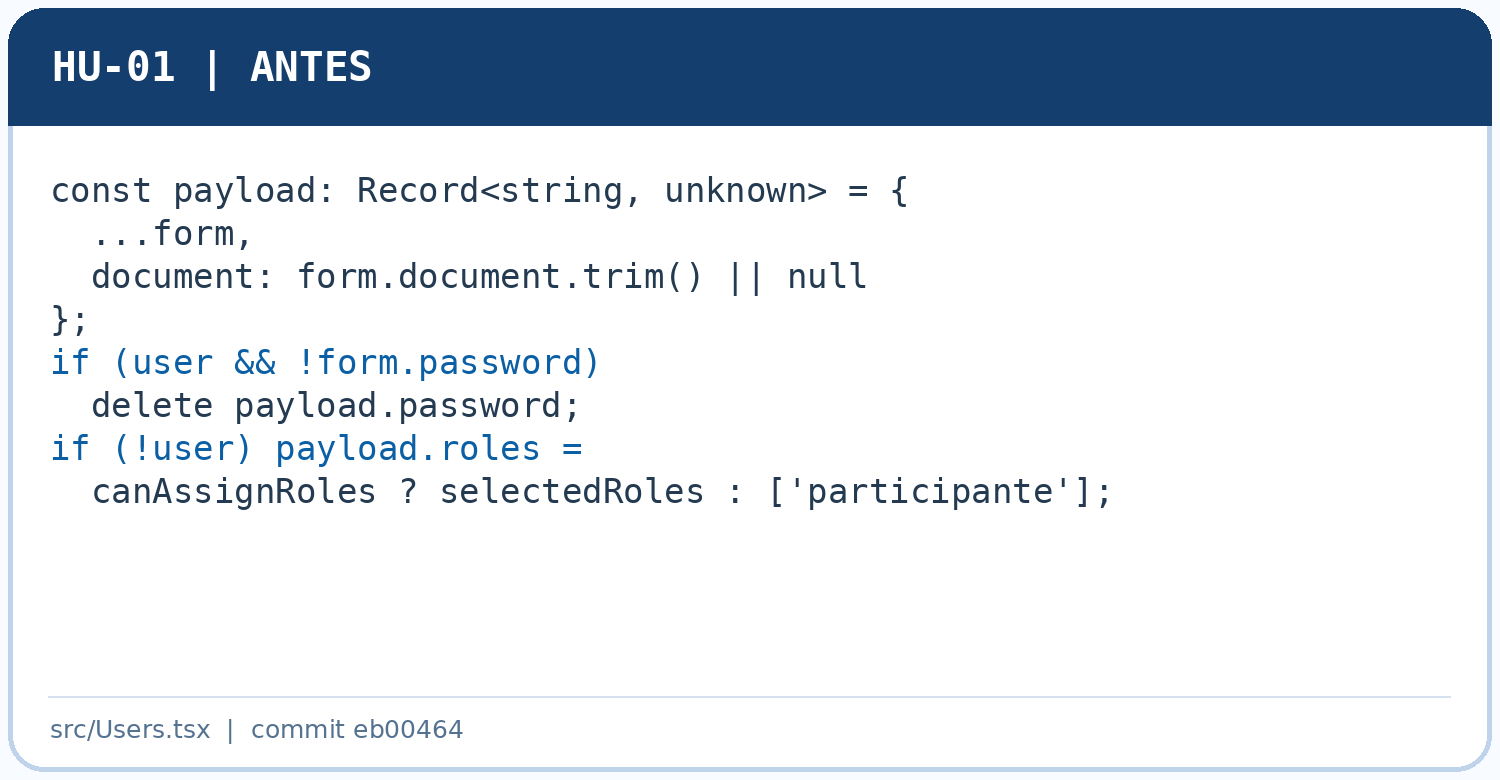
\includegraphics[width=0.90\linewidth]{imagenes/HU01_antes.png}
  \column{0.493\textwidth}
  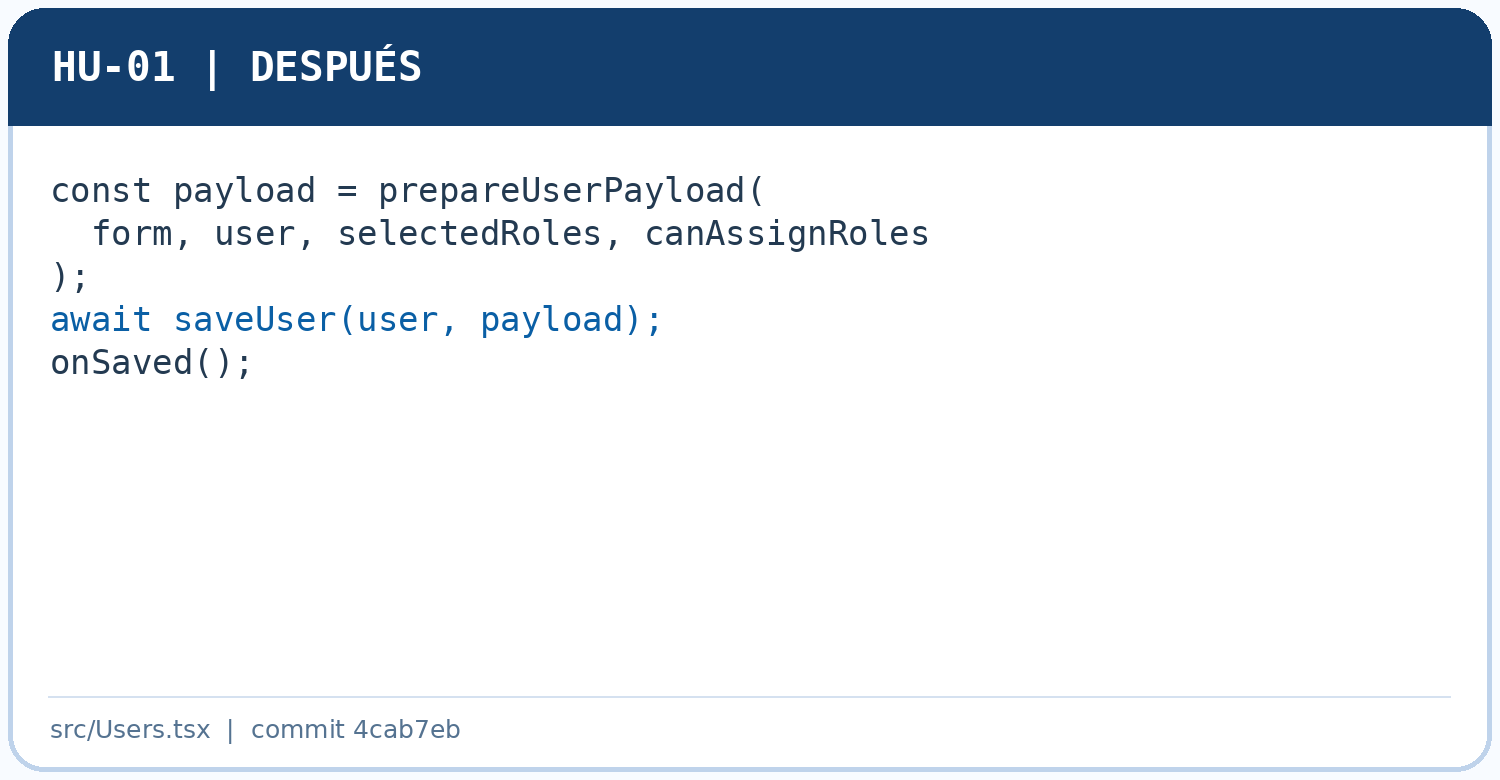
\includegraphics[width=0.90\linewidth]{imagenes/HU01_despues.png}
  \end{columns}
  \vspace{0.03cm}
  \cajaclara{\footnotesize \textbf{Qué cambió:} la preparación del \texttt{payload} y la petición HTTP se extrajeron de \texttt{submit()} a funciones específicas.\\
  \textbf{Por qué:} responsabilidad única, cohesión y menor acoplamiento.}
  \vspace{0.12cm}
  {\tiny Los extractos conservan la lógica del repositorio; saltos de línea adaptados para legibilidad. Fuente: commits \texttt{eb00464} y \texttt{4cab7eb}.}
\end{frame}

\begin{frame}{HU-02 | Roles y permisos: antes y después}
  \vspace{0.12cm}
  \begin{columns}[T,onlytextwidth]
  \column{0.493\textwidth}
  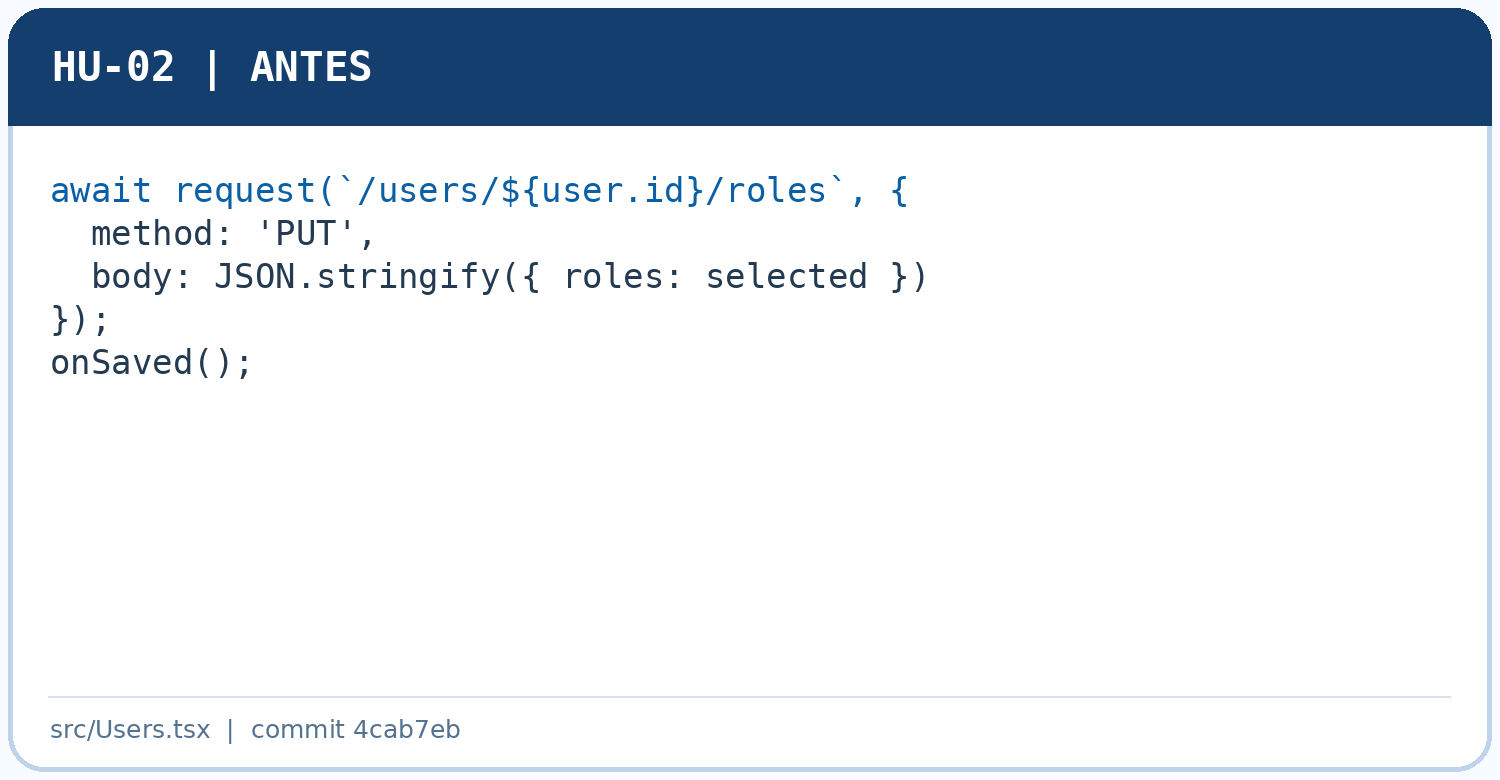
\includegraphics[width=0.90\linewidth]{imagenes/HU02_antes.png}
  \column{0.493\textwidth}
  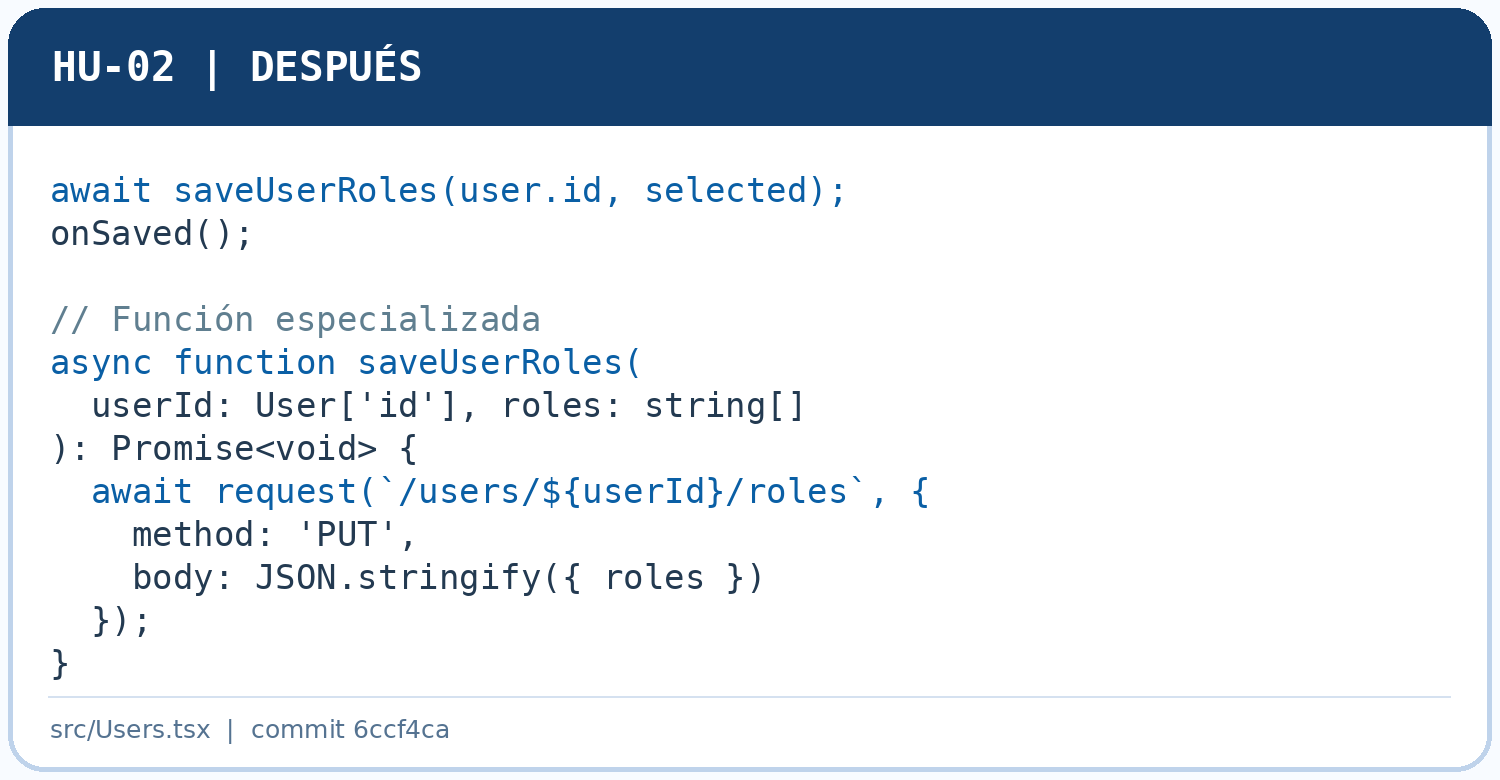
\includegraphics[width=0.90\linewidth]{imagenes/HU02_despues.png}
  \end{columns}
  \vspace{0.03cm}
  \cajaclara{\footnotesize \textbf{Qué cambió:} \texttt{UserRolesForm} usa \texttt{saveUserRoles()}; también se separaron \texttt{saveRolePermissions()}, \texttt{toggleSelection()} y \texttt{loadRoleCatalog()}.\\
  \textbf{Por qué:} reutilización, menor duplicación y separación entre vista y acceso a datos.}
  \vspace{0.12cm}
  {\tiny Extractos basados en los commits \texttt{4cab7eb} y \texttt{6ccf4ca}; líneas ajustadas para la diapositiva.}
\end{frame}

\begin{frame}{Brenda | Verificación y trazabilidad}
  \begin{columns}[T,onlytextwidth]
  \column{0.46\textwidth}
  \begin{block}{Pruebas automáticas del proyecto}
    \vspace{0.18cm}
    {\centering\Huge\bfseries 28\par}
    {\centering\small pruebas aprobadas\par}
    \vspace{0.12cm}
    {\centering\Large\bfseries 0 fallidas\par}
    \vspace{0.14cm}
    {\centering\scriptsize \texttt{npm run check} | TypeScript + Vite OK\par}
  \end{block}
  \column{0.51\textwidth}
  \textbf{Comprobaciones manuales}\par\vspace{0.15cm}
  \begin{itemize}\setlength\itemsep{0.19cm}
    \item Registro de un usuario de prueba.
    \item Asignación de múltiples roles.
    \item Edición de permisos de un rol.
  \end{itemize}
  \vspace{0.20cm}
  \cajaclara{\footnotesize Las \textbf{28 pruebas} son de todo el sistema, principalmente backend. No se presentan como 28 pruebas exclusivas del frontend.}
  \end{columns}
\end{frame}

% RESPONSABLE: ADEL. Sustituir estos espacios por cambios y evidencia reales.
\begin{frame}{Adel | Backend de capacitaciones}
\begin{columns}[T,onlytextwidth]
\column{0.56\textwidth}
{\large\bfseries Apartado pendiente de integrar}\par\vspace{0.26cm}
\begin{itemize}\setlength\itemsep{0.22cm}
\item Identificar funciones o módulos realmente refactorizados.
\item Insertar imagen del código ANTES y DESPUÉS.
\item Explicar principio SOLID o patrón justificado.
\item Anotar prueba y commits verificables.
\end{itemize}
\column{0.40\textwidth}
\cajaclara{\textbf{HU-03 / HU-04}\\[0.12cm]Gestión de capacitaciones, backend y arquitectura.\\[0.24cm]\textit{State: candidato; documentar solo si existe implementación real.}}
\end{columns}
\end{frame}

% Evidencia local del 18/11/2026; no atribuye commits ni revisión humana pendientes.
\begin{frame}{Franshesco | Usuarios, autenticación y permisos}
\begin{itemize}
\item Base: Punto Inicio Fran, etiqueta \texttt{punto-inicio-fran}, commit \texttt{98f8d5a}; ya incluye a Brenda y Adel.
\item Antes: validación, reglas, hashing y SQL reunidos en usuarios y login.
\item Después: validadores, políticas, casos de uso y repositorios específicos.
\item SRP: responsabilidades separadas. DIP: servicios reciben repositorios, reloj, hashing, auditoría y transacción.
\item Permisos comprobados en servidor y revalidados después de esperar el hash; se conserva el último administrador activo.
\end{itemize}
\small Entrega: \texttt{Punto final fran 1} en \texttt{dev/franshesco}. Los rótulos sin commit describen capturas previas al cierre. Se conservan contratos y reglas de los compañeros.
\end{frame}

\begin{frame}{Franshesco | Observer con un consumidor real}
\begin{itemize}
\item Capacitaciones publica hechos mediante un puerto \texttt{events}; no conoce al servicio de avisos.
\item Un observador crea avisos internos para gestores e instructor asignado, según acceso vigente.
\item Transacción 1: capacitación, auditoría y evento pendiente. Publicación después del commit.
\item Transacción 2: avisos y evento procesado. Fallo: pendiente recuperable, sin avisos parciales.
\item Reintento manual hasta 50 eventos; unicidad evento/destinatario evita duplicados internos.
\end{itemize}
\small Observer organiza suscriptores; outbox conserva eventos. HU-26 parcial, sin WhatsApp, correo, worker ni tiempo real. Destinatarios pendientes de confirmar.
\end{frame}

\begin{frame}{Franshesco | Cómo se comprobó}
\begin{itemize}
\item Antes: 75 pruebas backend y cuatro casos Chrome. Después: 95 y cinco, aprobados localmente.
\item Casos: registro simultáneo, rollback, revocación durante hashing, propiedad/CSRF, fallo de observador, reintento y reinicio.
\item Listado de 100 entre 404 cuentas ficticias: 302 SELECT antes y cuatro después, excluyendo autenticación; no es una prueba de carga.
\item Nueve imágenes de código con versión, archivo, líneas y hashes.
\item Demostración: programar, abrir Avisos, modificar, actualizar y marcar como leído.
\end{itemize}
\small Pruebas aisladas. Fuentes y guion en \texttt{docs/franshesco/}. Revisión humana, cliente e integración por PR pendientes.
\end{frame}

% RESPONSABLE: DANIELA. Sustituir contenido por archivos y pruebas reales.
\begin{frame}{Daniela | Frontend de capacitaciones y calidad}
\begin{columns}[T,onlytextwidth]
\column{0.56\textwidth}
{\large\bfseries Apartado pendiente de integrar}\par\vspace{0.26cm}
\begin{itemize}\setlength\itemsep{0.22cm}
\item Mostrar refactorización de los formularios de capacitación.
\item Agregar fragmentos ANTES y DESPUÉS.
\item Justificar desacoplamiento y reutilización.
\item Incorporar pruebas funcionales y commits.
\end{itemize}
\column{0.40\textwidth}
\cajaclara{\textbf{Enfoque}\par\vspace{0.10cm}Interfaz de capacitaciones, validaciones y pruebas.\\[0.24cm]\textit{Strategy: evaluar solo si hay estrategias reales distintas.}}
\end{columns}
\end{frame}

\begin{frame}{Cierre y próximos pasos del equipo}
  \begin{columns}[T,onlytextwidth]
    \column{0.55\textwidth}
    {\Large\bfseries Entrega grupal coherente}\par\vspace{0.24cm}
    \begin{itemize}\setlength\itemsep{0.23cm}
      \item Una plantilla para todos los integrantes.
      \item Comparaciones basadas en commits reales.
      \item Justificaciones técnicas y pruebas verificables.
      \item Integración por Pull Request a \texttt{main}.
    \end{itemize}
    \column{0.41\textwidth}
    \cajaclara{\textbf{Antes de exponer}\par\vspace{0.16cm}Sustituir las tres secciones pendientes, revisar los PDF y confirmar con el equipo los resultados y patrones realmente implementados.}
  \end{columns}
\end{frame}

\end{document}